\usetikzlibrary{calc}
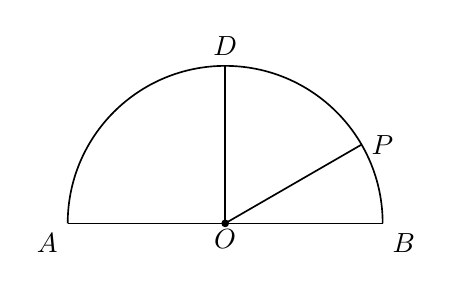
\begin{tikzpicture}[x=1cm,y=1cm,line width=.6pt,font=\normalsize]
\coordinate (O) at (0,0);
\coordinate (A) at (-2.0,0);
\coordinate (B) at (2.0,0);
\coordinate (D) at (0,2.0);
\coordinate (P) at (1.7321,1.0);
\draw (A) arc[start angle=180,end angle=0,radius=2cm];
\draw (A)--(B);
\draw (O)--(D);
\draw (O)--(P);
\node[below left] at (A) {$A$};
\node[below=2pt,inner sep=0pt] at (O) {$O$};
\node[below right] at (B) {$B$};
\node[above] at (D) {$D$};
\node[right] at (P) {$P$};
\fill (O) circle[radius=1.4pt];
\end{tikzpicture}
